\documentclass[review]{vgtc}

\graphicspath{{figures/}{pictures/}{images/}{./}}

% Keep the VR template's metrics and line spacing; only add Unicode/CJK fonts.
\usepackage{times}
\renewcommand*\ttdefault{txtt}
\usepackage{mathptmx}
\usepackage{fontspec}
\usepackage{xeCJK}
\setmainfont{Times New Roman}
\setsansfont{Arial}
\setmonofont{Courier New}
\setCJKmainfont[BoldFont=SimHei,ItalicFont=KaiTi]{SimSun}
\setCJKsansfont{Microsoft YaHei}
\setCJKmonofont{FangSong}

\usepackage{amsmath}
\usepackage{amssymb}
\usepackage{enumitem}
\hyphenation{Static-Lock Ego-Anchor}
\usepackage{array}
\usepackage{booktabs}
\usepackage{multirow}
\usepackage{tabularx}
\usepackage{xcolor}
\usepackage{placeins}

\onlineid{1118}
\vgtccategory{System}
\vgtcinsertpkg

% XeLaTeX/xdvipdfmx 下禁用嵌套链接，避免官方模板的脚注正文丢失。
\hypersetup{nesting=false}

% 仅将 URL 改为接近官方模板的窄体等宽字体，避免脚注地址过度换行。
\newfontfamily\EgoUrlMono{Latin Modern Mono}
\renewcommand{\UrlFont}{\EgoUrlMono}

\title{EgoAnchor：透视混合现实中日常物体的零样本动态锚定}

\author{%
  Hailin Ji 
  \thanks{e-mail: \texttt{jihailin@mail.bnu.edu.cn}} \\
  School of Artificial Intelligence \\
  Beijing Normal University \\
  Beijing, China
  \and Yifeng Chen 
  \thanks{e-mail: \texttt{yfchen@mail.bnu.edu.cn}} \\
  School of Artificial Intelligence \\
  Beijing Normal University \\
  Beijing, China
  \and Haonian Wang
  \thanks{e-mail: \texttt{haonianwang@mail.bnu.edu.cn}} \\
  School of Artificial Intelligence \\
  Beijing Normal University \\
  Beijing, China
  \and Yiran Zhang 
  \thanks{e-mail: \texttt{zhangyiran@mail.bnu.edu.cn}} \\
  School of Artificial Intelligence \\
  Beijing Normal University \\
  Beijing, China
  \and Hongwen Zhang 
  \thanks{Corresponding author; e-mail: \texttt{zhanghongwen@bnu.edu.cn}} \\
  School of Artificial Intelligence \\
  Beijing Normal University \\
  Beijing, China
  \and Yanhong Luo 
  \thanks{Corresponding author; e-mail: \texttt{273961431@xbmu.edu.cn}} \\
  College of Electrical Engineering \\
  Northwest Minzu University \\
  Lanzhou, China
}

\abstract{%

零样本6DoF位姿估计已能定位更多具备三维模型的日常刚性物体，但其异步、低频且质量波动的输出仍难直接作为稳定对象锚点。本文提出EgoAnchor，一套面向透视混合现实的第一人称零样本动态物体锚定系统。感知后端产生带视觉一致性评分的相机系位姿观测；运行时将观测恢复为采集时刻的世界系状态并维护面向渲染的可靠对象状态，使低频视觉输出形成稳定、连续且可恢复的锚点。我们在Meta Quest 3上实现系统，并通过以平台追踪为参考的受控基准评测、关键设计分析与24名参与者的被试内研究进行评价。结果显示，EgoAnchor的静态配准误差、遮挡恢复误差和时延对齐后的动态轨迹残差均更低，代价是更高的起动时延；用户研究进一步显示更高的主观静止稳定性、依赖意愿与信任。代码将随论文发表开源。
}

\keywords{透视混合现实, 动态物体锚定, 6DoF 位姿估计, 运行时系统, 用户感知。}

% ===== Teaser =====
\teaser{%
  \centering
  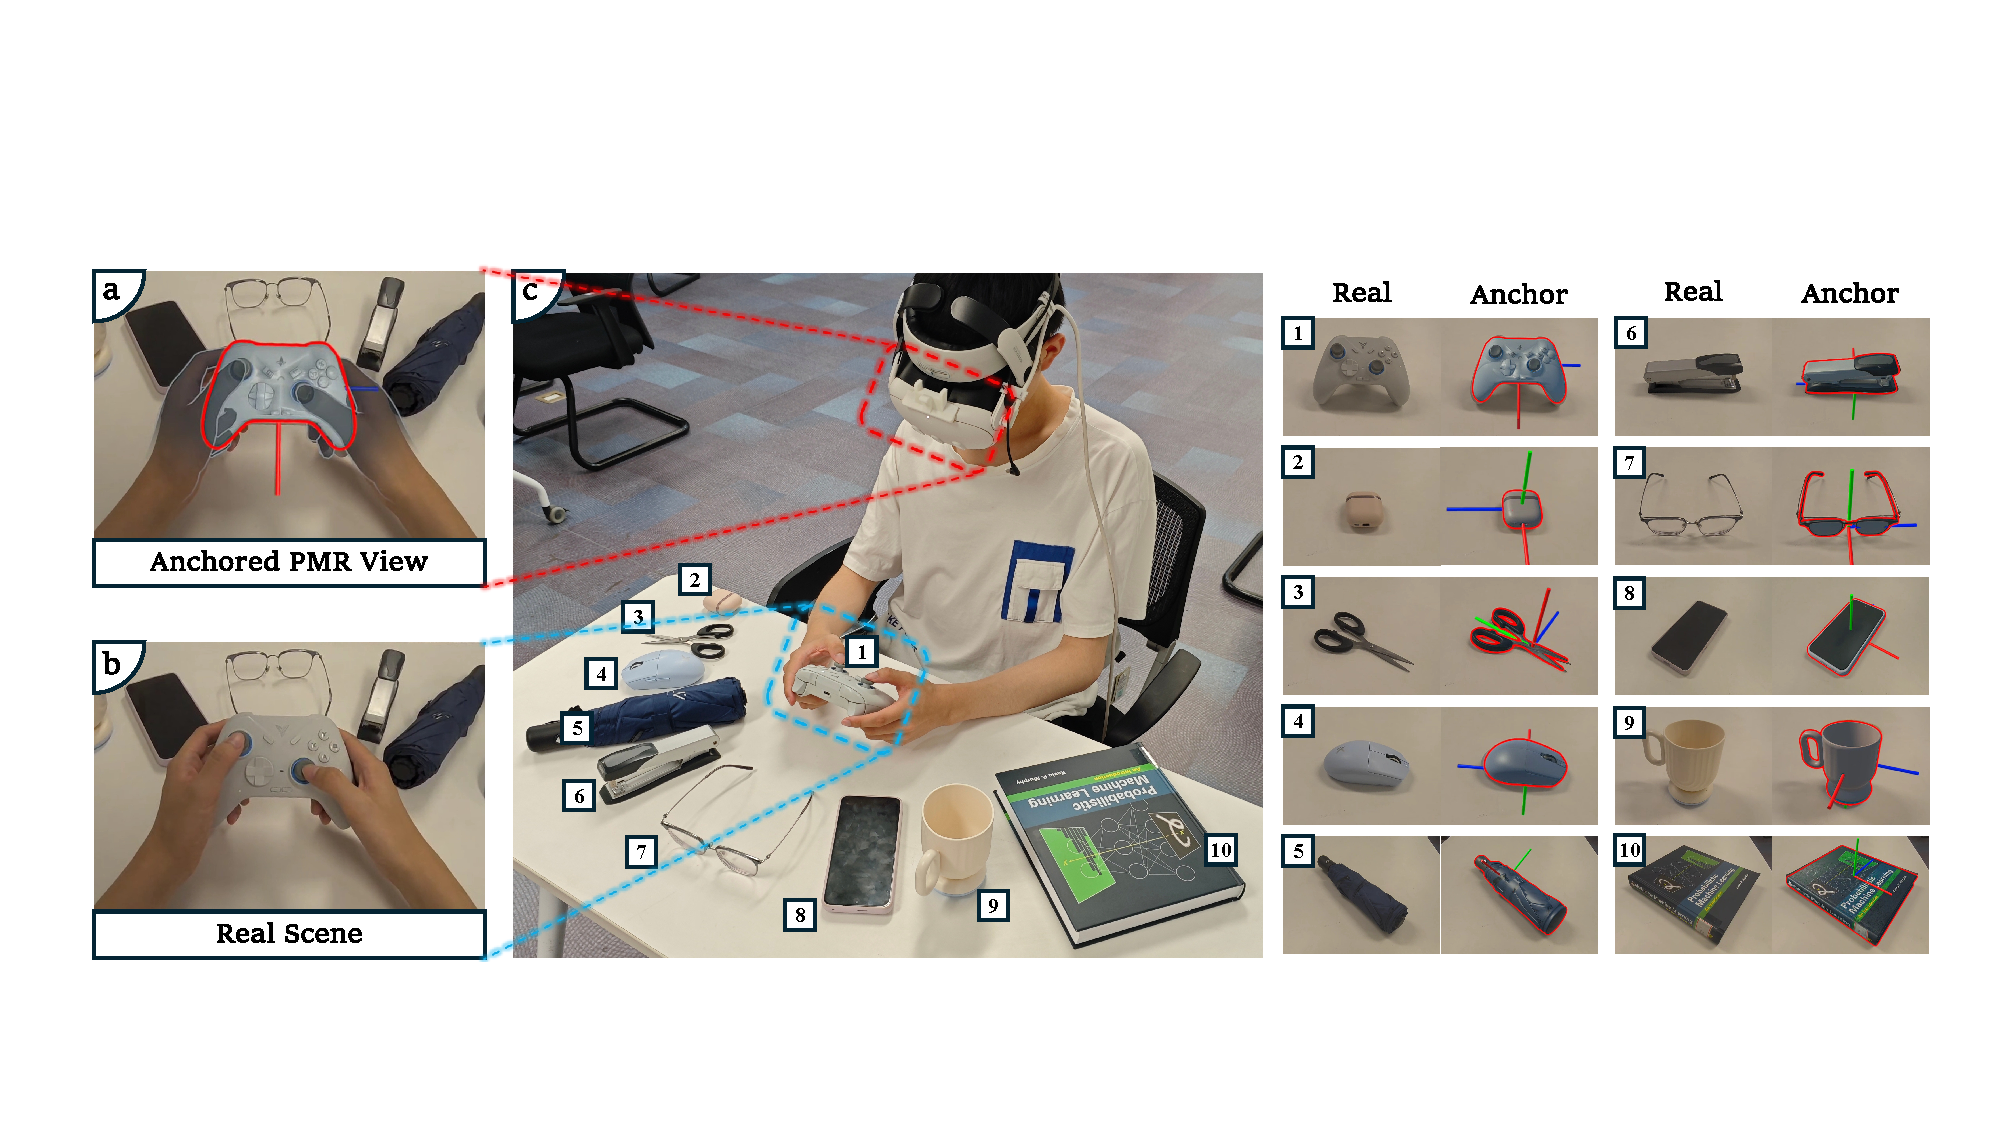
\includegraphics[width=\linewidth]{figures/teaser.pdf}
  \caption{EgoAnchor 在日常物体上的零样本动态锚定示例。(a) 第一人称锚定增强画面，(b) 同一时刻未增强的透视画面，(c) 第三人称交互视角。场景编号 1--10 与右侧十个物体对应；每组展示真实物体（Real）与 EgoAnchor 锚定可视化（Anchor）。红色轮廓与局部坐标轴表示估计的 6DoF 对象锚点。十个物体依次为游戏手柄、耳机盒、剪刀、无线鼠标、雨伞、订书机、眼镜、手机、马克杯和书本，覆盖不同尺度、几何与外观。}
  \label{fig:teaser}
}

\begin{document}

\firstsection{引言}\label{sec:introduction}
\maketitle

% ===== 第一段：问题动机 =====
透视混合现实（Passthrough Mixed Reality, PMR）将虚拟内容附着到用户身边的真实物体，用于物体说明、操作引导、状态可视化与近物交互。这类应用不仅需要识别物体，还需要随物体运动持续更新的对象级空间参考：用户转头、拿起、旋转、放下或短暂遮挡物体时，虚拟内容仍应保持一致的六自由度（6DoF）关系。传统空间锚点适合静态环境，却不能表达物体自身运动，因此动态物体锚定是以物体为中心的消费级混合现实应用的基础系统能力~\cite{selfblending2026,gradualreality2024}。

% ===== 第二段：现有方案局限 =====
现有方案在不同层面提供部分支持。平台原生对象追踪集成良好，但对象范围、模型准备与运行时行为由平台定义（如Apple Vision Pro、Meta Quest系列）；物理标记和专用追踪器稳定，却需改造或装备目标物体。近年来的开放词表检测、时序分割、立体匹配与模型驱动零样本6DoF估计使更多具有三维模型的刚性物体可被视觉定位~\cite{groundingdino2025,cutie2024,fastfoundationstereo2026,foundationpose2024,gigapose2024}。这些组件共同扩展了视觉定位范围，但最终位姿仍是与图像采集时刻绑定的相机系观测，而非MR应用可持续绑定的对象锚点。

% ===== 第三段：核心问题 =====
直接将视觉位姿作为对象锚点会暴露若干运行时问题。首先，异步结果到达时已滞后；若与到达时刻的头显位姿复合，头动会被错误写入物体世界位置。其次，候选即使经过时间对齐，仍可能因遮挡、深度噪声或几何错配而不准确，接纳后产生可见跳变。最后，低频、不规则且含噪的位姿流无法直接支撑逐帧渲染，运行时还需显式管理静止、运动、转换、短时观测失效与重新获取等状态行为。因此，单帧位姿精度不足以定义可持续使用的对象锚点。

% ===== 第四段：EgoAnchor解决方案 =====
因此，本文提出EgoAnchor，一套面向透视混合现实的零样本动态物体锚定系统。感知后端将开放词表检测、时序分割、双目深度与零样本位姿估计组织为持续流水线，并以逐观测可视度门控颜色--深度评分（Visibility-gated Color-Depth, VCD）估计候选可靠性。锚定运行时将异步候选恢复为采集时刻的世界系观测，并维护面向渲染的可靠对象状态，使系统在运动、静止与短时观测中断期间持续生成可供应用使用的对象锚点。新目标无需物理标记或逐物体训练，仅需三维模型与简短文本描述；三维模型可采用已有数字资产，或由图像离线生成。

% ===== 第五段：贡献（压缩） =====
本文的主要贡献为：
\begin{enumerate}[leftmargin=1.8em,itemsep=1pt,topsep=2pt]
  \item \textbf{EgoAnchor系统：}将异步、低频且质量波动的相机系零样本视觉观测转化为可用的世界系动态对象锚点。
  \item \textbf{锚定感知与运行时：}以VCD评估逐观测可靠性，并通过采集时刻对齐、时间索引状态与静止锚定维持连续、可恢复的运行时输出。
  \item \textbf{系统评价：}通过以平台追踪为参考的受控基准评测、关键设计分析与24名参与者的被试内研究，量化系统性能、设计取舍及其感知效用。
\end{enumerate}

\section{相关工作}\label{sec:related-work}

\subsection{MR物体锚定}

物体锚定为真实物体建立对象级空间参考，使虚拟内容能够持续附着。早期方法主要依赖AprilTag、ArUco等人工标记获得物体位姿~\cite{apriltag2011,aruco2014}，但需要改造目标物体，难以覆盖开放场景中的多类日常物体。

近年来，消费级混合现实平台开始提供免标记对象识别与追踪能力。Azure Object Anchors\footnote{\href{https://learn.microsoft.com/en-us/dynamics365/mixed-reality/guides/pc-app-anchor-object}{Azure Object Anchors}}、Vuforia Model Targets\footnote{\href{https://developer.vuforia.com/library/vuforia-engine/images-and-objects/model-targets/model-targets/}{Vuforia Model Targets}}、Apple Vision Pro\footnote{\href{https://developer.apple.com/documentation/visionos/implementing-object-tracking-in-your-app}{Apple object tracking}}以及Meta Quest\footnote{\href{https://developers.meta.com/horizon/documentation/native/android/mobile-dynamic-object-tracker/}{Meta dynamic object tracking}}等平台均可借助设备感知与目标模型建立对象级空间状态，但通常依赖预先生成的平台参考对象、离线目标配置，或受到对象类型与平台接口支持范围的限制。学术研究则进一步将头显的设备追踪、空间映射、相机与深度感知结合，用于场景资产定位、已知物体注册以及持续对象追踪~\cite{fan2021assettracking,doughty2022hmdegopose,pollabauer2023hololens,martingomez2024sttar,trojak2025mixedpose,greene2025markerless,trojak2026markerless,gbot2024}。这些工作验证了头显感知与对象级追踪结合的可行性，但通常仍依赖特定对象、任务先验、专用硬件或平台配置，对开放场景中多类日常物体的灵活接入支持有限~\cite{hurt2025surrealitycv}。

\subsection{6DoF物体位姿估计与追踪}

6DoF物体位姿估计从视觉观测中恢复刚性物体相对于相机的空间位姿，是动态物体锚定的重要感知基础~\cite{aguirrezabal2026survey}。相关研究已从依赖局部几何特征的传统方法，发展到利用RGB-D融合、稠密几何回归、对称性建模和自监督学习的已知实例估计~\cite{densefusion2019,epos2020,gdrnet2021,self6d2020}，并进一步扩展到未见物体与零样本场景~\cite{gen6d2022,megapose2022,lin2024sam6d,ornek2024foundpose,moon2025coop,foundationpose2024}。与此同时，滤波与多帧几何方法可以维持跨帧对象状态~\cite{poserbpf2021,bundletrack2021}。

视觉基础模型进一步扩大了开放场景中的对象感知范围：开放词表检测允许通过文本语义指定目标~\cite{owlvit2022,glip2022,groundingdino2025,yoloe2025}，视频对象分割能够维持帧间对象身份~\cite{xmem2022,cutie2024}，现代双目匹配则提升了复杂场景下的深度恢复与跨域泛化~\cite{raftstereo2021,igevstereo2023,fastfoundationstereo2026}。这些能力共同使面向日常物体的零样本视觉定位逐渐可行，但主要解决相机坐标系中的感知与位姿估计问题；在混合现实中，视觉观测仍需进一步转化为稳定、连续的世界系对象状态，才能形成可持续使用的对象锚点。

\subsection{XR时间对齐}

XR系统中的感知、追踪与传输通常引入处理时延，使渲染时可用的状态对应早于当前显示的观测时刻；端到端时延还会随系统负载与处理过程发生变化~\cite{diluca2010latency,mrloop2022,stauffert2020mtp}。针对这种状态与目标时刻之间的时间错位，一类典型方法是\emph{预测式追踪（predictive tracking）}：根据历史运动将已有状态预测或外推至当前或预期显示时刻，以减小由追踪与显示时延造成的动态配准误差~\cite{azuma1994improving,laviola2003double,pvt2023,yoon2022headmotion}。

另一种做法是保留状态的时间戳，并按指定的历史时刻查询或重建状态。已有AR系统通过时间戳、采样时刻调整以及插值或外推实现不同延迟数据流之间的时间配准~\cite{jacobs1997latency}。OpenXR进一步区分未来状态预测与\emph{历史状态查询（history query）}：未来时刻由运行时预测，而过去时刻依据所保留的历史状态返回相应估计。因此，预测式追踪用于减小状态滞后，而历史状态查询用于恢复指定过去时刻的空间状态，两者体现了不同的时间对齐方式。

\section{EgoAnchor系统}\label{sec:system}

\subsection{系统概览}

EgoAnchor以简短文本描述与离线三维模型指定目标，无需物理标记或逐物体训练。感知后端持续形成带可靠性评分的相机系位姿观测，锚定运行时恢复其采集时刻对应的世界位姿，并按渲染节奏维护对象锚点。

运行时显式区分图像采集时刻$t_f$、候选到达时刻$t_a$与渲染时刻$t_r$。全文以$T_a^b\in\mathrm{SE}(3)$表示从坐标系$a$到$b$的刚体变换，$w,c,o$分别表示世界、左目相机与对象坐标系；滤波状态与应用输出分别记为$\widehat{T}$与$\widetilde{T}$。图~\ref{fig:arch}展示系统职责与异步数据流。

\begin{figure*}[t]
  \centering
  
\includegraphics[width=\textwidth]{figures/pipeline.pdf}
  \caption{EgoAnchor 架构与异步数据流。感知后端由双目图像、文本描述和三维模型完成语义初始化、时序分割、深度恢复与零样本 6DoF 位姿估计，并以可视度（V）、颜色（C）和深度（D）计算 VCD 可靠性。异步观测 $o_f$ 到达运行时后按采集时刻恢复世界位姿，经准入与状态更新形成时间索引轨迹 $B_j$；渲染帧在 $t_q$ 查询轨迹，并在运动追踪/静止锚定间切换。可靠观测持续缺失时重新获取。}

  \label{fig:arch}
\end{figure*}

\subsection{感知后端}\label{sec:perception}

\textbf{输入与目标。}
给定头显双目图像$I_f = (I_f^L, I_f^R)$、目标的文本描述$Q_o$与三维模型$G_o$，感知后端为每个处理帧形成观测
\begin{equation}
o_f = (f, t_f, T_{o,f}^{c}, R_f),
\label{eq:observation}
\end{equation}
其中$f$为头显端分配的帧标识，$T_{o,f}^{c}$为目标在该帧左目相机坐标系中的位姿，$R_f \in [0,1]$为逐观测可靠性评分。序列$\{o_f\}$构成连接两层的异步观测流。

\subsubsection{面向锚定的感知流水线}

流水线依次建立目标身份、米制深度与相机系位姿。

\textbf{语义初始化。}
开放词表检测器~\cite{yoloe2025}在初始化帧$f_0$由左目图像与文本描述获得目标掩膜：
\begin{equation}
M_{f_0} = \operatorname{Detect}(I_{f_0}^{L}, Q_o),
\label{eq:detect}
\end{equation}
其中$f_0$为首次同时取得有效掩膜与足够深度覆盖的帧，重新获取时重新指定。

\textbf{时序分割。}
初始掩膜用于初始化视频对象分割器~\cite{cutie2024}，此后逐帧传播目标身份：
\begin{equation}
(M_f, H_f) = \operatorname{Seg}(I_f^{L}, H_{f-1}), \qquad f > f_0,
\label{eq:seg}
\end{equation}
其中$H_f$为时序外观记忆，使位姿估计持续作用于同一目标实例。

\textbf{双目深度恢复。}
立体匹配器由校正后的双目图像预测视差并恢复米制深度：
\begin{equation}
d_f = \operatorname{Stereo}(I_f^{L}, I_f^{R}), \qquad Z_f = \frac{b f_x}{d_f},
\label{eq:depth}
\end{equation}
其中$b$与$f_x$分别为双目基线和像素焦距。

\textbf{零样本位姿估计。}
模型驱动估计器~\cite{foundationpose2024}由掩膜、深度与三维模型恢复相机系位姿：
\begin{equation}
T_{o,f}^{c} =
\begin{cases}
\operatorname{Reg}(M_f, Z_f, G_o), & \text{注册}, \\
\operatorname{Track}(M_f, Z_f, G_o, T_{o,f^-}^{c}), & \text{追踪},
\end{cases}
\label{eq:pose}
\end{equation}
注册仅在初始化与重新获取时执行，连续帧采用前一结果初始化的局部追踪。

\subsubsection{逐观测VCD评分}

零样本位姿优化可能产生与当前观测不一致的候选。VCD沿用渲染--观测比较范式~\cite{deepim2018,latentfusion2020,focalpose2022}，以可视度（V）、颜色（C）与深度（D）证据评估每个候选。

\textbf{可视度门控。}
记$M_f^{\mathrm{rnd}}$为候选位姿下的渲染掩膜，则
\begin{equation}
\Omega_f = M_f \cap M_f^{\mathrm{rnd}}, \quad \Omega_f^{\circ} = \operatorname{Erode}(\Omega_f), \quad V_f = \frac{|\Omega_f|}{|M_f^{\mathrm{rnd}}|},
\label{eq:visibility}
\end{equation}
其中$V_f$衡量渲染投影获得观测支持的比例，核心区$\Omega_f^\circ$用于排除边界混合像素。

\textbf{颜色与深度一致性。}
颜色一致性$S_f^C$采用LAB空间的零均值归一化互相关并降低亮度通道权重。深度一致性结合距离自适应的绝对残差项$S_f^{D,\mathrm{abs}}$和对整体深度偏置更鲁棒的结构项$S_f^{D,\mathrm{str}}$：
\begin{equation}
S_f^D = (1-\alpha_f)\,S_f^{D,\mathrm{abs}} + \alpha_f\,S_f^{D,\mathrm{str}},
\label{eq:depth-score}
\end{equation}
其中$\alpha_f$为两项之间的深度变化相关权重。平坦目标主要依赖绝对深度，而几何起伏明显的目标获得更强的结构约束。

\textbf{证据聚合。}记$K_f\subseteq\{C,D\}$为本帧有效模态集合，则
\begin{equation}
R_f = V_f \cdot
\begin{cases}
\exp\!\left(\dfrac{\sum_{k \in K_f} w_k \ln \max(S_f^{k}, \epsilon)}{\sum_{k \in K_f} w_k}\right), & K_f \neq \varnothing, \\[6pt]
1, & K_f = \varnothing.
\end{cases}
\label{eq:vcd}
\end{equation}
其中$w_k$为模态权重，$\epsilon$为对数下限。无效模态不参与聚合；若颜色与深度均不可用，评分退化为$V_f$。乘性可视度门控使遮挡或投影错位直接降低候选可靠性。

\subsection{锚定运行时}\label{sec:anchoring}

锚定运行时将低频异步候选流转化为与显示刷新同步的对象状态：候选到达时恢复采集时刻的世界位姿并更新轨迹，渲染帧则从轨迹合成锚点，并依据运动与观测支持管理静止锚定和有效性。候选事件与渲染事件分离，使输出频率不受感知到达率限制。

\subsubsection{观测校正}\label{sec:obs-update}

运行时先按采集时刻恢复候选的世界系位姿，再执行可靠性/时序准入并更新状态轨迹。

\textbf{观测对齐。}
候选$T_{o,f}^{c}$对应采集时刻$t_f$，但于$t_a$返回；若使用到达时刻相机位姿，期间头动会被写入对象位置。运行时以帧标识$f$缓存采集时刻的$T_{c,f}^{w}$，候选返回后计算
\begin{equation}
T_{o,f}^{w} = T_{c,f}^{w}
\begin{bmatrix}
1 & 0 & 0 & 0 \\
0 & -1 & 0 & 0 \\
0 & 0 & 1 & 0 \\
0 & 0 & 0 & 1
\end{bmatrix}
T_{o,f}^{c}
\begin{bmatrix}
-1 & 0 & 0 & 0 \\
0 & 1 & 0 & 0 \\
0 & 0 & 1 & 0 \\
0 & 0 & 0 & 1
\end{bmatrix},
\label{eq:capture-alignment}
\end{equation}
其中两个固定矩阵分别处理视觉/渲染坐标约定及其对象局部坐标轴约定之间的差异。

\textbf{可靠准入。}
第$j$个接纳观测记为$(t_j,T_{o,j}^{w},R_j)$。首个候选满足可靠性门槛即可建立轨迹，后续候选还须保持采集时刻递增：
\begin{equation}
R_f \geq R_{\min}, \qquad t_f > t_j \quad (j \geq 1).
\label{eq:admission}
\end{equation}
被拒候选不更新状态。

\textbf{状态更新。}
每个接纳观测触发平移与旋转的常速度卡尔曼更新~\cite{kalman1960new}，得到$\widehat{T}_{o,j}^{w}$及时间索引轨迹
\begin{equation}
B_j = \{(t_i, \widehat{T}_{o,i}^{w})\}_{i=1}^{j}.
\label{eq:trajectory}
\end{equation}
同一更新同步刷新静止锚定所需的运动与可靠性证据。

\subsubsection{锚点合成}\label{sec:frame-output}

轨迹$B_j$低频且不规则，渲染需逐帧得到对象状态。运行时先选择历史查询时刻$t_q$，再由相邻轨迹节点插值。

\textbf{历史查询。}
最新节点时刻$t_j$相对渲染时刻$t_r$的状态年龄为$\ell_r=t_r-t_j$，运行时根据其非对称指数估计$\bar{\ell}_r$设置查询滞后：
\begin{equation}
\ell_r = t_r - t_j, \qquad \Delta_r = \max(\Delta_{\min},\, s\,\bar{\ell}_r), \qquad t_q = t_r - \Delta_r.
\label{eq:target-time}
\end{equation}
其中，$\Delta_{\min}$为最小查询滞后，$s$为缩放因子，$t_q$为用于状态重建的历史查询时刻。该策略使$t_q$尽量落在两个可用轨迹节点之间。

\textbf{状态插值。}
当查询时刻满足 $t_i\leq t_q\leq t_{i+1}$ 时，运行时在相邻轨迹节点之间对物体状态进行插值：

\begin{equation}
\lambda_q = \frac{t_q - t_i}{t_{i+1} - t_i}, \qquad
\widehat{T}_o^w(t_q) = \operatorname{Interp}(\widehat{T}_{o,i}^{w}, \widehat{T}_{o,i+1}^{w}; \lambda_q),
\label{eq:history-interp}
\end{equation}

其中，位置采用线性插值，旋转采用 SLERP。对于超出可用轨迹范围的查询时刻，运行时保持最近端点状态。

\textbf{输出模式。}为抑制静止期残余波动，EgoAnchor在追踪与锁定之间切换：
\begin{equation}
\widetilde{T}_o^w(t_r) = \begin{cases}
\widehat{T}_o^w(t_q), & \text{追踪}, \\
T_{o,\mathrm{lock}}^w, & \text{锁定}.
\end{cases}
\label{eq:staticlock}
\end{equation}

\subsubsection{静止锚定}\label{sec:staticlock}

我们设计了静止锚定机制 StaticLock，用于在持续低运动且可靠的观测条件下将输出切换为锁定位姿，并在检测到明确物体运动或可靠性下降时释放锁定状态。

\textbf{进入。}由相邻接纳观测计算并指数平滑平移/旋转速率$\bar v_j,\bar\omega_j$，定义
\begin{equation}
\sigma_j = \max\left(\frac{\bar{v}_j}{v_{\mathrm{th}}},\ \frac{\bar{\omega}_j}{\omega_{\mathrm{th}}}\right), \qquad \sigma_j \leq 1, \qquad R_j \geq R_{\mathrm{lock}}.
\label{eq:lock-entry}
\end{equation}
条件持续$\tau_{\mathrm{dwell}}$后，以当前追踪位姿初始化$T_{o,\mathrm{lock}}^w$；同时冻结低通观测共识为参考$T_{o,\mathrm{ref}}^w$，用于度量累计漂移。

\textbf{锁定状态更新。}
设 $d_{p,j}$ 和 $d_{\theta,j}$ 分别表示当前观测与锁定位姿之间的平移和旋转残差。基于死区阈值 $d_{\mathrm{db}}$ 和 $\theta_{\mathrm{db}}$，定义
$\delta_j=\max(d_{p,j}/d_{\mathrm{db}},d_{\theta,j}/\theta_{\mathrm{db}})$。
锁定位姿更新为：
\begin{equation}
T_{o,\mathrm{lock},j}^w =
\begin{cases}
\operatorname{Interp}\left(T_{o,\mathrm{lock},j-1}^w, T_{o,j}^{w};\, g_j\right), & \delta_j \leq 1, \\
T_{o,\mathrm{lock},j-1}^w, & \delta_j > 1.
\end{cases}
\label{eq:lock-update}
\end{equation}
其中，$g_j$ 为由观测可靠性决定的更新增益。死区范围内的变化通过较慢更新逐步吸收，而超出死区的偏移则作为释放锁定状态的依据。

\textbf{释放。}持续死区外残差、相对$T_{o,\mathrm{ref}}^w$的累计漂移、持续明确运动或可靠性下降任一成立时，系统在下一渲染帧退回追踪；运动判据随头动强度适度放宽，以降低视角变化造成的误释放。

\textbf{有效性与重新获取。}\label{sec:validity}
锚点按近期可靠观测支持标记为有效、不确定或丢失：短时缺失时继续查询轨迹并在必要时保持最后可信位姿，超时后停止交付。若锚点丢失或候选持续低可靠，后端重新注册并重置状态、轨迹与锁定状态，由首个新接纳观测开始新的追踪段。

% 原3.4“运行流程”与图2及上述事件路径重复，已删除。

\section{系统实现}\label{sec:implementation}

EgoAnchor两层通过局域网通信。感知后端运行于NVIDIA RTX 5090工作站，基于Python 3.14.6/PyTorch 2.12.1/CUDA 13.2/TensorRT 11.1实现；运行时基于Unity 6000.3.11f1与Meta XR SDK 203.0.0，经Quest Link运行于Intel i9-14900K/32~GB主机。Quest 3负责双目采集、设备追踪与显示。

\textbf{感知后端。}
后端使用YOLOE-26初始化开放词表目标~\cite{yoloe2025}，Cutie传播掩膜~\cite{cutie2024}，Fast-FoundationStereo恢复米制深度~\cite{fastfoundationstereo2026}，FoundationPose执行零样本6DoF注册/追踪~\cite{foundationpose2024}；VCD借助nvdiffrast渲染模型~\cite{nvdiffrast2020}。RTX 5090上追踪阶段服务器处理时间中位数/P95为75.44/88.47~ms，候选到达率中位数13.25~Hz；全部定量结果均来自该配置。

\textbf{锚定运行时。}
运行时以C\#实现，通过Meta Passthrough Camera API获取双目图像与相机标定，并以帧标识缓存相机位姿历史。所有运行时阈值与增益在三个实验中保持固定；完整参数配置随代码与补充材料提供。

\textbf{通信。}
双目图像与相机标定通过ZeroMQ/Protobuf传输并采用最新帧优先，位姿、状态与控制消息通过NATS Core/Protobuf传输。图像与返回观测保留一致的帧标识，用于运行时恢复对应采集时刻的相机位姿。

\section{评估设计}\label{sec:evaluation}
我们通过三个互补实验评价EgoAnchor：实验一在受控条件下比较四种运行时配置的静态、动态与转换行为；实验二分别分析采集时刻对齐、静止锚定、VCD可靠性排序以及预测与历史查询的取舍；实验三以日常刚性物体开展被试内研究，考察主观锚定质量、信任与依赖。

日常物体三维模型由Hunyuan3D~\cite{hunyuan3d22025tencent}从手机照片生成并经网格简化/纹理重烘焙；Quest 3控制器采用官方资产。

\subsection{实验一：应用侧锚点行为}\label{sec:exp1-design}

\textbf{参考与场景。}
评价以Quest 3控制器为视觉追踪目标，并以平台SDK的同步6DoF位姿作为追踪参考。四类采集场景覆盖对象锚定的主要运行状态：静止目标下的主动头动、静止与6DoF运动间的起停切换、连续平移/旋转，以及完全遮挡后的重新显露，分别用于考察静态稳定性、转换响应、动态跟随与遮挡恢复。

\textbf{比较条件。}
四种配置接收同一原始候选流。\textbf{Arrival}/\textbf{Capture}直接保持最新候选，仅在世界系复合时分别使用到达/采集时刻。\textbf{One-Euro}~\cite{casiez2012oneeuro}作为自适应平滑基线，对与EgoAnchor相同的接纳观测进行速度自适应低通滤波，维护用于逐帧输出的时间索引轨迹，但不启用静止锚定。该滤波器以较低计算开销和较少参数在抖动抑制与响应滞后之间折中。\textbf{EgoAnchor}为完整系统。

\textbf{评价指标。}
九项指标分三组：\textbf{静态配准}包括头动泄漏（观察者运动引入的相对变化）、配准误差（相对平台追踪参考的空间偏差）和静止抖动（相邻帧增量）；\textbf{动态跟随}包括有效时延（使回移参考与输出残差最小的时延）、LA-RMSE（该最小残差）、CT-RMSE（未作时延对齐的当前时刻误差）和残余抖动（对齐残差的高频分量）；\textbf{转换响应}包括遮挡误差（遮挡开始至稳定恢复）和运动起动时延（参考运动开始至锚点响应）。除运动起动时延为跨通道标量外，其余均分平移/旋转报告。

\subsection{实验二：设计分析}\label{sec:exp2-design}

实验二针对四项关键设计开展有针对性的归因分析。

\textbf{观测对齐。}
同一相机系候选分别按图像采集时刻与候选到达时刻恢复世界位姿，比较主动头动条件下的位姿泄漏，评价时间语义恢复对静态配准的影响。

\textbf{静止锚定。}
在完整EgoAnchor上关闭静止锚定，比较静止条件下的头动泄漏，评价其对静止期锚点稳定性的贡献。

\textbf{VCD。}
候选按VCD评分排序，并以风险--覆盖率曲线下面积（AURC）概括评分与平移误差之间的排序关系~\cite{riskcontrolled2020,ding2020uncertainty}；AURC越低，表示较高VCD评分越优先选择低误差候选。

\textbf{预测与历史查询。}
为量化响应速度--轨迹保真的取舍，我们比较\emph{预测式追踪}与\emph{历史状态查询}。前者以平滑卡尔曼常速度模型外推至$t_r$，并衰减校正残差以保持连续；后者按第~\ref{sec:frame-output}~节在$t_q$对已到达相邻节点执行平移线性插值与旋转SLERP。两者共享候选流、状态估计与准入规则。

\subsection{实验三：用户研究}\label{sec:exp3-design}

实验三进一步考察受控评价中的系统差异是否反映到用户感知。我们在日常刚性物体上比较One-Euro与完整EgoAnchor，重点测量静止稳定性、运动附着、遮挡恢复以及用户对锚点的信任与依赖。

\subsubsection{实验设计}

研究选择视觉可观测性与操作遮挡互补的无线鼠标、订书机和游戏手柄，覆盖弱纹理曲面、细长多平面以及较丰富几何/纹理与自然抓握遮挡。采用完全被试内设计，每位参与者在三个物体上分别体验One-Euro与EgoAnchor；条件评分在参与者内跨物体取均值，物体与方法顺序平衡，并以匿名A/B标签呈现。

\subsubsection{任务}

每个方法--物体条件依次完成三项标准化操作：静止观察；拿起物体完成约25--30~cm平移与30--45°自然旋转后放置；以及用统一挡板完全遮挡约1~s后观察恢复。三项任务连续完成后统一评分。

\subsubsection{主观测量}

主观测量包括七项对象锚定条目，以及Augmentation Quality（AQ）、Trust in Automation（TiA）与S-TIAS三个已发表量表。

\textbf{对象锚定条目。}
七项条目均采用七点同意度量表，覆盖实验一考察的应用侧行为，并参考AR追踪与信任研究~\cite{trustar2024}：阶段行为包括静止稳定、运动附着、姿态一致和恢复一致，整体判断包括位置正确、依赖意愿和稳定--响应平衡。各条目分别分析而不合并总分；完整措辞见补充材料。

% 原Table 1（七项对象锚定条目完整措辞）移至补充材料。

\textbf{增强质量（AQ）。}
采用AQ~\cite{aq2026}的嵌入质量（EQ）与交互质量（IQ）两个完整三条目子量表，分别评价虚实嵌入以及操作时的交互质量，均为七点同意度。

\textbf{用户信任（TiA与S-TIAS）。}
TiA~\cite{tia2019}采用可靠性/能力六项与理解/可预测性四项（五点同意度），S-TIAS~\cite{stias2025}以三个七点条目给出总体信任分。量表仅对指代对象作情境化改编，中文译文经逐条核对并在预实验认知访谈中检查可理解性。

最终问卷另记录总体方法偏好、信任选择、偏好强度、方法区分信心与实验后不适情况，均只作描述性报告。

\subsubsection{实验流程}

研究获作者所属机构伦理审查批准，参与者签署知情同意。完成背景问卷、头显调整与练习后，参与者依次体验六个方法--物体条件，每个条件后完成对象锚定条目与AQ；全部条件结束后分别评价两种方法的TiA与S-TIAS并填写最终问卷。单次实验约60分钟，可按需休息。

\subsubsection{参与者}

共招募24名参与者并全部纳入分析（20--36岁，$M=27.08$，$\mathrm{SD}=4.45$；女性/男性各12名；22名右利手）。其中6名从未使用VR/MR，10名使用过1--5次，8名至少6次；12名无真实物体AR/MR操作经验。

\subsubsection{统计分析}

七项对象锚定条目与AQ-EQ/IQ先在参与者内跨三个物体取均值，TiA两分量表与S-TIAS按方法分别计算得分，共12项结局。各结局报告Mdn [Q1,Q3]；24组完整配对采用双侧条件精确Wilcoxon符号秩检验，并报告匹配秩双列相关$r_{\mathrm{rb}}$及参与者级自举95\%置信区间。七项自定义条目与五项已发表量表结局分别构成两个Holm校正家族；已发表量表另按方法报告Cronbach's $\alpha$。

\section{结果}\label{sec:results}

\subsection{实验一：应用侧锚点行为}

结果按第~\ref{sec:exp1-design}~节三类指标报告。表~\ref{tab:exp1-static}--\ref{tab:exp1-transition}汇总中位数，图~\ref{fig:exp1-final}给出重复采集的分布，图~\ref{fig:exp1-replay}展示连续回放。指标先在单次序列内汇总，再取重复间中位数；双通道按平移/旋转报告。

\begin{figure*}[!t]
  \centering
  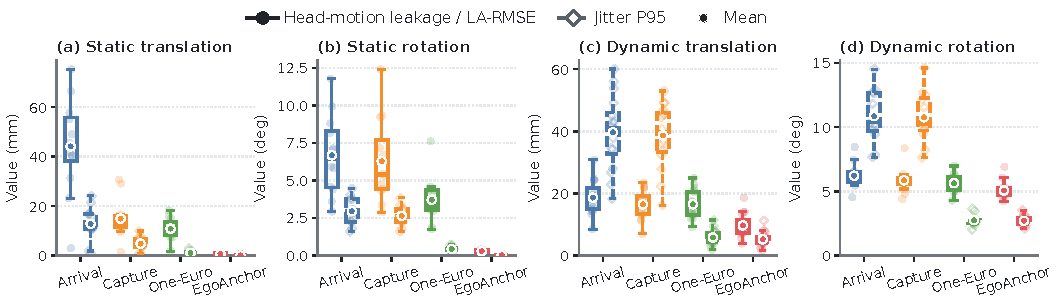
\includegraphics[width=\textwidth]{figures/panels/figure2_exp1_behavior.pdf}
  \caption{实验一四种配置的误差分布：(a,b)静止平移/旋转，报告头动泄漏与静止抖动P95；(c,d)持续运动平移/旋转，报告LA-RMSE与残余抖动P95。浅色点为重复采集，箱体/横线为IQR/中位数，深色点为均值；均为越低越好。EgoAnchor静态误差最接近零、LA-RMSE最低，动态残余抖动与One-Euro相近。}

  \label{fig:exp1-final}
\end{figure*}

\subsubsection{静态配准}

\begin{table}[t]
\centering
\caption{实验一静态配准。单元格按平移/旋转给出重复测量中位数，三项均为P95；$\downarrow$越低越好，粗体为通道最优，分布见图~\ref{fig:exp1-final}(a,b)。}
\label{tab:exp1-static}
\begin{tabular}{@{}lccc@{}}
\toprule
方法 & \shortstack{头动泄漏\,$\downarrow$\\mm/$^\circ$} & \shortstack{配准误差\,$\downarrow$\\mm/$^\circ$} & \shortstack{静止抖动\,$\downarrow$\\mm/$^\circ$} \\
\midrule
Arrival & 43.67/6.49 & 44.31/9.65 & 11.70/2.98 \\
Capture & 13.03/5.40 & 17.54/8.26 & 4.30/2.60 \\
One-Euro & 10.65/3.29 & 14.00/6.96 & 0.85/0.40 \\
EgoAnchor & \textbf{0.82}/\textbf{0.33} & \textbf{6.60}/\textbf{4.39} & \textbf{0.06}/\textbf{0.03} \\
\bottomrule
\end{tabular}
\end{table}

主动头动首先暴露了异步观测的时间语义问题。Arrival的头动泄漏达到43.67~mm/6.49°；将同一候选按图像采集时刻解释后，Capture降至13.03~mm/5.40°。One-Euro为10.65~mm/3.29°，EgoAnchor为0.82~mm/0.33°，相较One-Euro在两个通道上分别降低约92\%和90\%；配准误差呈同向排序，最低值同样由EgoAnchor取得（6.60~mm/4.39°）。静止抖动上，两种直接保持最新候选的配置仍有可见波动，One-Euro降至0.85~mm/0.40°，EgoAnchor为0.06~mm/0.03°，比One-Euro再低一个数量级以上；图~\ref{fig:exp1-final}(a,\,b)显示其静止输出集中在接近零的窄范围内。

\subsubsection{动态跟随}

\begin{table}[t]
\centering
\caption{实验一动态跟随。单元格按平移/旋转给出重复测量中位数；残余抖动为P95，$\downarrow$越低越好，粗体为通道最优，分布见图~\ref{fig:exp1-final}(c,d)。}
\label{tab:exp1-dynamic}
\setlength{\tabcolsep}{2pt}
\begin{tabular}{@{}lcccc@{}}
\toprule
方法 & \shortstack{有效时延\,$\downarrow$\\ms} & \shortstack{LA-RMSE\,$\downarrow$\\mm/$^\circ$} & \shortstack{CT-RMSE\,$\downarrow$\\mm/$^\circ$} & \shortstack{残余抖动\,$\downarrow$\\mm/$^\circ$} \\
\midrule
Arrival & \textbf{202.5}/\textbf{255.0} & 18.57/6.09 & \textbf{84.74}/25.44 & 41.08/10.40 \\
Capture & 255.0/257.5 & 17.14/5.84 & 103.63/\textbf{25.35} & 39.69/10.26 \\
One-Euro & 380.0/385.0 & 15.69/5.55 & 117.61/34.10 & 5.25/2.70 \\
EgoAnchor & 360.0/345.0 & \textbf{9.12}/\textbf{4.81} & 125.83/31.88 & \textbf{4.56}/\textbf{2.64} \\
\bottomrule
\end{tabular}
\end{table}

按各方法自身的最佳有效时延对齐后，LA-RMSE反映去除整体响应滞后后的轨迹残差。EgoAnchor的LA-RMSE为9.12~mm/4.81°，相较One-Euro的15.69~mm/5.55°分别降低约42\%和13\%；残余抖动为4.56~mm/2.64°与5.25~mm/2.70°。相比静止条件，两种方法在残余抖动上的差距较小，而LA-RMSE的差异更为明显。

当前时刻行为呈现不同的排序。直接保持候选的配置滞后较低（Arrival 202.5/255.0~ms），采用状态估计与历史状态查询后升至One-Euro的380.0/385.0~ms与EgoAnchor的360.0/345.0~ms。若不作时延对齐，该滞后会计入当前时刻误差：CT-RMSE的平移分量由Arrival的84.74~mm增至EgoAnchor的125.83~mm，旋转分量则以EgoAnchor的31.88°低于One-Euro的34.10°。因此，较低的LA-RMSE并不意味着当前时刻配准误差同步降低。

\subsubsection{转换响应}

\begin{table}[t]
\centering
\caption{实验一转换响应。遮挡误差按平移/旋转给出重复测量中位数（P95），运动起动时延为跨通道标量；$\downarrow$越低越好，粗体为最优。}
\label{tab:exp1-transition}
\begin{tabular}{@{}lcc@{}}
\toprule
方法 & \shortstack{遮挡误差\,$\downarrow$\\mm/$^\circ$} & \shortstack{运动起动\,$\downarrow$\\ms} \\
\midrule
Arrival & 18.23/18.39 & \textbf{157.0} \\
Capture & 16.93/18.38 & 263.8 \\
One-Euro & 10.41/8.66 & 334.0 \\
EgoAnchor & \textbf{4.85}/\textbf{5.52} & 510.4 \\
\bottomrule
\end{tabular}
\end{table}

表~\ref{tab:exp1-transition}把遮挡恢复与起动响应并列。短时完全遮挡期间，遮挡误差由Arrival的18.23~mm/18.39°与One-Euro的10.41~mm/8.66°降至EgoAnchor的4.85~mm/5.52°，相较One-Euro分别降低约53\%和36\%。运动起动时延由Arrival的157.0~ms、One-Euro的334.0~ms增加至EgoAnchor的510.4~ms，其排序与遮挡误差相反。

\subsubsection{定性回放}

\begin{figure}[t]
  \centering
  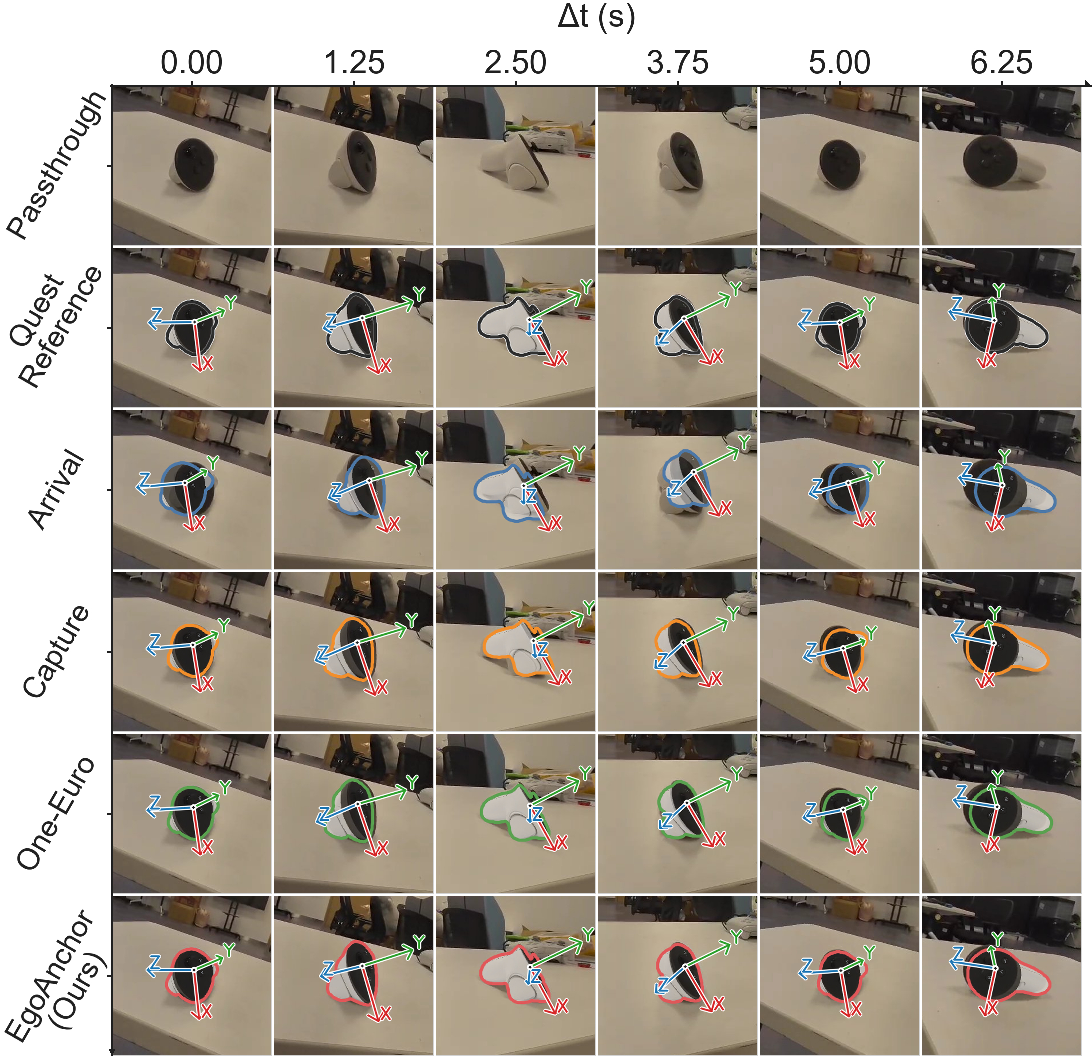
\includegraphics[width=\columnwidth]{figures/replay_grid.pdf}
  \caption{实验一连续序列回放（$\Delta t=0$--$6.25\,\mathrm{s}$，间隔$1.25\,\mathrm{s}$）。上两行为原始透视图像与Quest平台追踪参考，下四行为Arrival、Capture、One-Euro、EgoAnchor在相同采集时刻的锚点投影；轮廓和局部轴表示估计6DoF锚点，用于比较头动/物体运动下的配准与时间连续性。}
  \label{fig:exp1-replay}
\end{figure}

图~\ref{fig:exp1-replay}展示这些定量差异在连续回放中的视觉表现：头动期间Arrival/Capture偏离更明显，One-Euro较小，EgoAnchor最接近平台追踪参考，与静态结果一致。

\subsection{实验二：设计分析}

实验二各项设计分析均使用独立采集的配对测量；每次重复先按指标汇总，再报告跨重复统计量，方括号为自举95\%置信区间，相对变化另报告配对比值。

\begin{figure*}[!t]
  \centering
  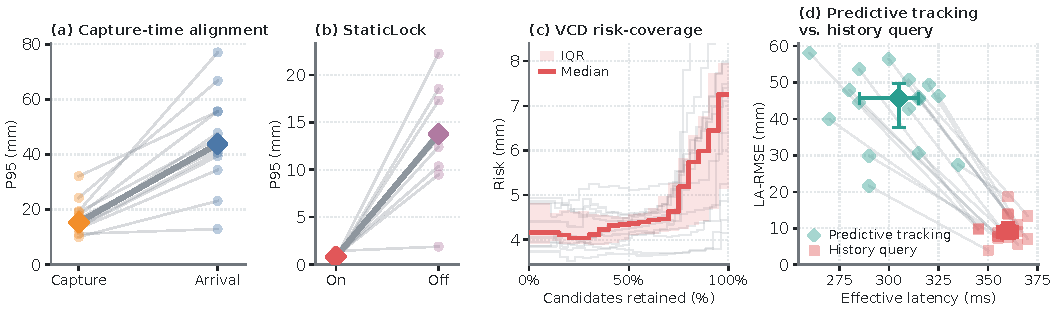
\includegraphics[width=\textwidth]{figures/panels/figure3_exp2_attribution.pdf}
  \caption{实验二四项设计分析：(a)采集/到达时刻复合的头动泄漏P95；(b)StaticLock开/关的头动泄漏P95；(c)VCD按分数保留候选的风险--覆盖率（红线/阴影：跨重复中位数/IQR）；(d)预测追踪与历史查询的有效时延--LA-RMSE。灰线连接配对序列。采集时刻对齐和StaticLock降低静态误差，高VCD分对应低风险；历史查询以更高时延换取更低轨迹残差。}
  \label{fig:exp2-final}
\end{figure*}

图~\ref{fig:exp2-final}(a,b)分别考察世界系复合所使用的时间语义与静止锚定。主动头动条件下，同一批相机系候选按图像采集时刻复合时，头动泄漏P95的中位数为15.38~mm；若改用候选到达时刻的相机位姿，该值升至43.75~mm，配对倍率为2.69 [2.38, 3.00]倍，表明采集时刻对齐本身即可大幅缩小由头动引入的空间错配。在完整EgoAnchor上仅关闭静止锚定后，静止条件下的头动泄漏P95由0.82~mm升至13.73~mm，对应17.06 [13.89, 27.52]倍的配对差异。该结果表明，静止锚定是静止期低波动输出的主要贡献因素。

图~\ref{fig:exp2-final}(c)以风险--覆盖率曲线考察VCD评分与候选误差的关系。按评分从高到低纳入候选时，高分候选对应较低的选择性风险，随着覆盖率提高并纳入更低分候选，风险逐步上升；遮挡条件下的AURC为4.79 [4.20, 5.13]~mm，全覆盖风险为7.25 [5.15, 7.95]~mm。该趋势表明VCD评分能够对候选几何误差提供有用的排序信息。

图~\ref{fig:exp2-final}(d)比较预测式追踪与历史状态查询的响应时延和轨迹残差。预测式追踪的有效时延为305.00/250.00~ms，低于历史状态查询的360.00/345.00~ms；但其时延对齐RMSE为45.64~mm/12.21°，而历史状态查询为8.93~mm/4.70°。按配对比值计算，预测条件的平移与旋转轨迹残差分别为历史查询条件的5.46 [4.02, 5.73]倍和2.63 [2.44, 2.78]倍。预测条件通过外推未观测运动获得更低的有效时延，而历史查询条件保留了更低的时延对齐轨迹残差。


\subsection{实验三：用户研究}

图~\ref{fig:exp3-subjective}展示24名参与者的配对评分；12项完整中位数、Wilcoxon统计量、Holm校正$p$值与效应量见补充材料，正文保留主要结果与关键非显著结果。

\begin{figure*}[!t]
  \centering
  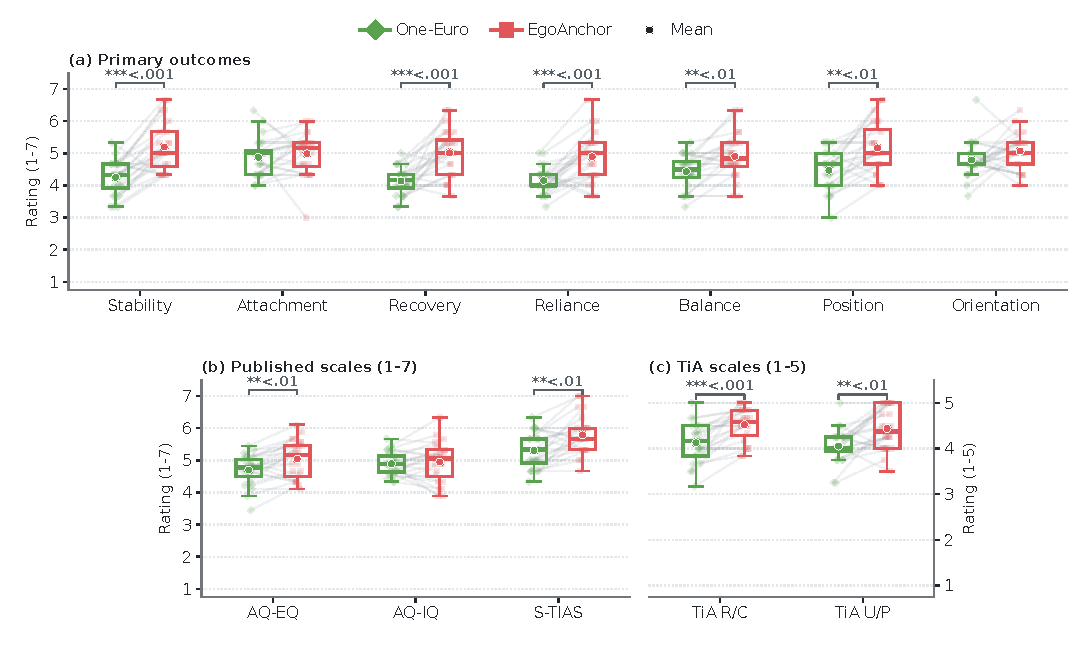
\includegraphics[width=\textwidth]{figures/panels/figure4_exp3_subjective_outcomes.pdf}
  \caption{24名参与者对One-Euro与EgoAnchor的被试内评价：(a)静止稳定、运动附着、姿态一致、恢复一致；(b)位置正确、依赖意愿、稳定--响应平衡；(c)AQ-EQ、AQ-IQ与S-TIAS；(d)TiA可靠性/能力（R/C）与理解/可预测性（U/P）。锚定条目与AQ先跨三个物体取均值；(a)--(c)为7点、(d)为5点评分。浅色点/灰线为个体/配对，箱体/横线/黑点为IQR/中位数/均值；星号为家族内Holm校正（$^*p_{\rm adj}<.05$，$^{**}<.01$，$^{***}<.001$）。}
  \label{fig:exp3-subjective}
\end{figure*}

% 原Table 5（实验三完整12项统计结果）移至补充材料。

\subsubsection{对象锚定体验}

\textbf{静止与恢复阶段。}
七项条目中两个较大的效应出现在这两个阶段。静止条件下，EgoAnchor的评分中位数为5.00 [4.58, 5.67]，高于One-Euro的4.33 [3.92, 4.67]，差异经Holm校正后成立（$W=13.5$，$p_{\mathrm{adj}}<.001$，$r_{\mathrm{rb}}=.90$）。遮挡移除后，EgoAnchor的恢复一致评分为5.00 [4.33, 5.42]，One-Euro为4.17 [3.92, 4.33]，对应七项条目中最大的效应量（$W=6$，$p_{\mathrm{adj}}<.001$，$r_{\mathrm{rb}}=.95$）。

\textbf{持续运动阶段。}
物体处于持续运动时，两种方法的主观差异明显减弱。运动附着评分为EgoAnchor 5.17 [4.58, 5.33]、One-Euro 5.00 [4.33, 5.08]；姿态一致评分为EgoAnchor 5.00 [4.67, 5.33]、One-Euro 4.67 [4.67, 5.00]。两项均未检测到Holm校正后的差异（附着：$W=67.5$，$p_{\mathrm{adj}}=.267$，$r_{\mathrm{rb}}=.29$；一致：$W=81$，$p_{\mathrm{adj}}=.162$，$r_{\mathrm{rb}}=.41$）。

\textbf{整体锚定判断。}
三项整体评价均偏向EgoAnchor。位置正确评分为EgoAnchor 5.00 [4.67, 5.75]、One-Euro 4.67 [4.00, 5.00]（$W=16$，$p_{\mathrm{adj}}=.001$，$r_{\mathrm{rb}}=.85$）；依赖意愿为EgoAnchor 5.00 [4.33, 5.33]、One-Euro 4.00 [4.00, 4.33]（$W=16.5$，$p_{\mathrm{adj}}<.001$，$r_{\mathrm{rb}}=.87$）；稳定--响应平衡为EgoAnchor 4.83 [4.58, 5.33]、One-Euro 4.50 [4.25, 4.75]（$W=6$，$p_{\mathrm{adj}}=.003$，$r_{\mathrm{rb}}=.90$）。

\subsubsection{增强质量与信任}

\textbf{增强质量。}
AQ的两个子量表显示，方法差异主要出现在嵌入质量而非交互质量。EgoAnchor的嵌入质量评分为5.17 [4.50, 5.47]，One-Euro为4.78 [4.50, 5.03]，差异经Holm校正后成立（$W=32$，$p_{\mathrm{adj}}=.004$，$r_{\mathrm{rb}}=.75$）。交互质量评分则彼此接近：EgoAnchor为5.06 [4.50, 5.33]，One-Euro为4.89 [4.64, 5.14]，未检测到校正后的显著差异（$W=102.5$，$p_{\mathrm{adj}}=.446$，$r_{\mathrm{rb}}=.19$）。

\textbf{用户信任。}
三项信任结局均为EgoAnchor评分更高。TiA可靠性/能力呈现最大的效应量（$W=0$，$p_{\mathrm{adj}}<.001$，$r_{\mathrm{rb}}=1.00$），EgoAnchor为4.58 [4.29, 4.83]，One-Euro为4.17 [3.83, 4.50]；理解/可预测性上，EgoAnchor为4.38 [4.00, 5.00]，One-Euro为4.00 [3.94, 4.25]（$W=32$，$p_{\mathrm{adj}}=.004$，$r_{\mathrm{rb}}=.75$）。S-TIAS总体信任上，EgoAnchor为5.67 [5.33, 6.00]，One-Euro为5.33 [4.92, 5.67]（$W=22.5$，$p_{\mathrm{adj}}=.004$，$r_{\mathrm{rb}}=.79$）。

One-Euro下AQ交互质量（.504）与TiA理解/可预测性（.565）的内部一致性较低，S-TIAS在两种方法下也相对偏低（.672/.697）。因此，对相应量表层面差异的解释需保持谨慎；完整Cronbach's $\alpha$见补充材料。

\textbf{总体选择。}
总体偏好也更倾向EgoAnchor：15/24（62.5\%）偏好EgoAnchor、4/24偏好One-Euro、5/24无明显偏好；直接信任选择为18/1/5。偏好强度中位数4.00 [3.00,5.00]，方法区分信心6.00 [5.00,7.00]；3人报告轻微不适，无人中止。

\section{讨论}\label{sec:discussion}

\subsection{技术启示}

综合各项评价，最明确的收益来自显式处理采集时刻语义与静止状态，而非仅依赖逐帧平滑。VCD进一步提供有用的可靠性排序，历史状态查询则以响应滞后换取更低的时延对齐轨迹残差。这些系统层面的差异也反映在位置正确、依赖意愿与信任评分上。在该问题设定下，可用的动态对象锚定因此需要将位姿、采集时刻、可靠性与异步到达组织为应用可持续使用的连续对象状态。

EgoAnchor以更低的静态误差、遮挡恢复误差和时延对齐轨迹残差换取更长的运动起动时延；持续运动时，其平移CT-RMSE高于One-Euro。用户评价的优势也主要集中于静止、恢复与整体依赖，而持续运动未检测到差异。因此，放置后查看、对象信息显示等任务可更重视稳定与轨迹保真，而快速连续操纵更需要降低响应滞后。

\subsection{局限与未来工作}

\textbf{对象与三维模型。}
EgoAnchor面向具有可用三维模型的刚性物体，其性能受目标可观测性与模型质量约束。严重遮挡、弱纹理、透明或镜面材质以及双目深度失效会削弱分割、深度恢复与位姿验证；非刚性对象超出本文的刚体位姿模型。由于同一三维模型同时参与位姿估计与VCD验证，其尺度、几何或坐标系误差会传递至锚点。图像到三维方法可简化模型获取，但生成模型质量仍会影响锚定。未来可研究面向锚定的模型生成、尺度校准与自动化流程。

\textbf{评价参考与跨平台比较。}
受控评价仅在Quest 3完成，尚缺跨头显6DoF比较。不同平台在对象模型、坐标约定、更新频率、时间戳与失效语义上可能不同，因此比较需统一对象坐标系、采样时刻与有效性。Quest 3控制器与头显共享世界坐标系并可建立固定对象坐标对应，但该参考仍依赖平台追踪而非独立真值。未来可结合外部光学动捕或机器人平台建立共同6DoF参考。

\textbf{部署与评价基准。}
当前实现依赖外部GPU工作站，感知与通信时延仍限制快速运动下的当前时刻配准质量；降低感知时延、提高候选频率以及向头显侧部署将扩大系统对快速操纵任务的适用范围。受控6DoF基准评测为保持同步追踪参考与固定对象坐标对应，仅使用Quest 3控制器；被试内研究选取三种刚性物体，以在对象多样性、单次实验时长与参与者疲劳之间取得平衡。未来可在更多对象与设备上复用静态配准、动态跟随和转换响应三类指标，进一步建立跨设备、跨对象的动态物体锚定基准~\cite{cheng2024tracking,hu2024applemeta,hu2025xrrealitycheck}。

\section{结论}\label{sec:conclusion}

本文提出EgoAnchor，一套面向透视混合现实的第一人称零样本动态物体锚定系统，将异步相机系观测恢复为采集时刻的世界系状态，并维持稳定、连续且可恢复的逐帧锚点。相较所评估基线，受控评价显示其静态配准与遮挡恢复误差更低、时延对齐轨迹残差更小，但运动起动时延更高；24名参与者的研究进一步显示更高的静止稳定性、恢复一致性、位置正确性、依赖意愿与信任评分。

将视觉位姿输出转化为对象级空间状态，不仅需要位姿精度，还需运行时显式处理观测时间、可靠性与逐帧输出。随着开放词表感知模型、三维生成与头显计算能力发展，感知--运行时协同有望将动态锚定扩展到更多日常物体与交互。

\acknowledgments{
  该研究得到中国国家自然科学基金项目（No. 62377004）的资助。
}

\bibliographystyle{abbrv-doi-hyperref-narrow}
\bibliography{egoanchor_cn_refs}

\end{document}
